\chapter{Object Reconstruction and Selection}

In this chapter I discuss the progression from detector-based signals through to an
overall event reconstruction within CMS. At CMS, physics-object reconstruction draws
on input from all detector subseystems simultaneously to build particle tracks
and cluster together energy deposits, to link together these tracks and energy
deposits to construct basic physics-objects such as electrons and charged
hadrons, and to build composit objects such as ``jets'' and hadronically decaying
$\tau$ leptons. Event based quantities such as the \etvecmiss are also reconstructed.
To achieve all of this, CMS uses its Particle Flow (PF) reconstruction 
algorithm~\cite{Sirunyan:2017ulk}. The particle flow concept has been used in the 
past by other experiments such as ALEPH at LEP~\cite{PF-ALEPH}. CMS is the first
experiment to fully utilize the particle flow techinque in a hadron collider environment.
A discussion of the reconstruction of the two basic PF objects, tracks and energy
clusters, follows in the next section. Afterwards I detail the construction of 
the PF physics-objects then move to the composit objects and full event variables.
The PF approach allows particles from pileup interactions to be identified 
and enables efficient pileup mitigation methods.

\section{Particle Flow Input}
The CMS detector and the PF reconstruction algorithm were specifically designed to
compliment eachother. The CMS detector features: a highly-segmented tracker well
suited to track reconstruction, a fine-grained electromagnetic calorimeter necessary
to separate the individual energy deposits from particles within ``jets'' and
efficient photon and electron identification, a hermetic hadron 
calorimeter for the measurement and identification of charged and neutral hadrons, 
a strong magnetic field for the measurement of the momenta of charged particles and to
separate the calorimeter energy deposits of charged and neutral hadrons within ``jets'', and 
an excellent muon spectrometer for muon identification and to disintangle the muon
tracks from other tracks in the tracker. A schematic of a slice of the CMS detector
and different physics-objects transversing the detector subsystems can be see in
figure~\ref{fig:cms_slice}. The different detector systems all contribute
necessary pieces of information to the PF reconstruction. From the raw detector
signals two classes of PF objects are created, tracks and energy clusters.

\begin{figure*}[htbp]
\centering
     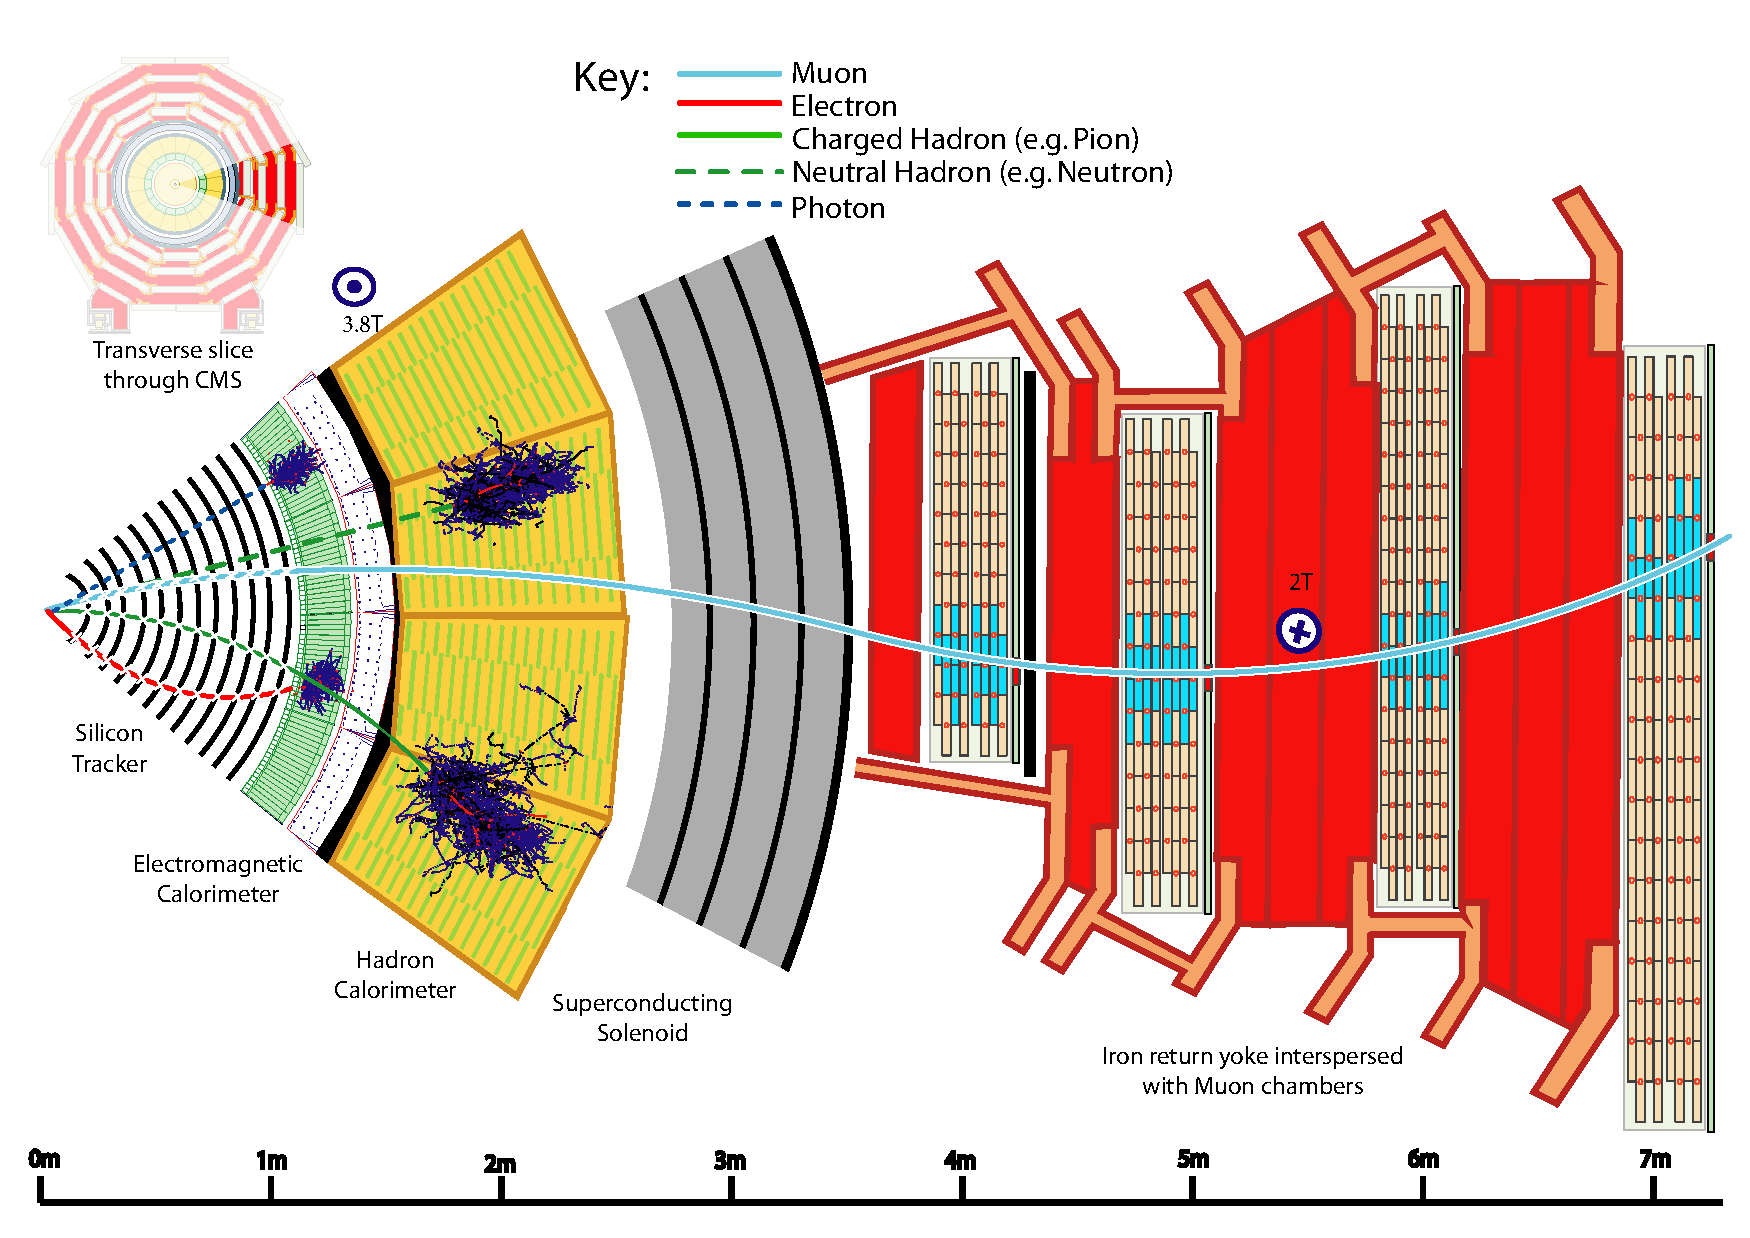
\includegraphics[width=1.0\textwidth]{object_reconstruction_and_selection/plots/cms_slice.pdf}
     \caption{
A schematic of a slice of an x-y cross section of the CMS detector showing different
physics-objects such as electrons, photons, charged and neutral hadroncs, and muons
propagating outwards from the collision region within the detector. The schematic
shows how tracks are linked to energy deposits and in which subdetector regions different
particles deposit most of their energy on average.
     }
     \label{fig:cms_slice}
\end{figure*}


\subsection{Particle Flow Tracks}
Energy deposits often called ``hits'' are recorded by the pixel and strip tracks during
a collision. From these, charged particle tracks are reconstructed in subsequent layers
mapping the progression of charged particles from the beam axis outwards into the detector
volume. Attempting to reconstruct tracks from every possible hit combination quickly
because unreasonable considering the over 70 million tracker pixels and strips which can
each record a hit. PF uses a combinatorial track finder based on Kalman 
Filtering (KF); the algorithim is broken down into three successive steps.
\begin{itemize}
\item Generate seed tracks from a few hits which are compatible with a charged
particle trajectory
\item Gathering other hits along the seed track trajectory when propagated through
the rest of the tracker subsystem
\item Final track fitting to determine track properties such as the origin, transverse
momentum, and direction.
\end{itemize}
Only tracks meeting certain quality standards are kept for analysis. These tracks must
be seeded with two hits in consecutive layers in the pixel detector, and are required 
to be reconstructed with at least eight tracker hits in total, and with at most one 
missing hit along the track trajectory. Tracks must also have a curvature corresponding
to a momentum greater than 0.9\GeV.

There is a balance that must be struck between imposing tight quality cuts on reconstructed
tracks which increases the purity of genuine track within the reconstructed track collection
but also decreases the efficiency for reconstructing genuine tracks, and loosening
quality cuts to reconstruct genuine tracks with a higher efficiency and lower purity.
After an initial pass through what is called the global combinatorial track finder,
which has stringent track quality criteria impossed by the eight hit requirement, 
the efficiency to reconstruct
genuine tracks is roughly 80\% for charged pions with $\pt = 10\GeV$, and 99\%
for isolated muons. This corresponds to a misreconstructed track rate in the range of
about 2.5\% for charged pions with $\pt = 10\GeV$, see figure~\ref{fig:kf_tracking}.
As hits are recorded in a reconstructed track, they are removed from the available,
unused hits which can be combined in subsequent passes through the tracking algorithm.

There are ten passes through the tracking algorithm in total. Each pass loosens the track quality criteria,
such as $\chi^2$ and number of hits requirements, beyond the stingent initial criteria.
This helps to reconstruct difficult to build tracks. Tracks can be difficult to 
reconstruct for multiple reasons such as detector inefficiencies leading to missing
detector hits, or particles originating from elsewhere in the detector 
besides along the beam axis. These tracks could be from hadrons interacting
within the tracker material before reaching the eight-hits threshold, or from the decay
of particles with finite life-times. Additionally, there can be difficulty disintangling
the many tracks within a collimated ``jet'' where many of the tracks are close to or
nearly overlapping with one another.
The misreconstruction rate is suppressed in each iterative step despite the loosening
quality criteria by the removal of the hits which are previously incorporated into
a reconstructed track. This  suppresses the random hit-to-seed association in the
next iteration and allows moderate efficiency gains for only small misreconstruction losses.
The efficiency and misreconstruction rate in figure~\ref{fig:kf_tracking} shows the
results for the initial pass throug the tracking algorithm, the results after all
passes which require the track seed to contain hits in the pixel detector, and the
final results after considering displaced tracks as well.
After all iterations the efficiency is about 90\% for a charged pions with $\pt = 10\GeV$
for a misreconstruction rate of 3\%.

\begin{figure*}[htbp]
\centering
     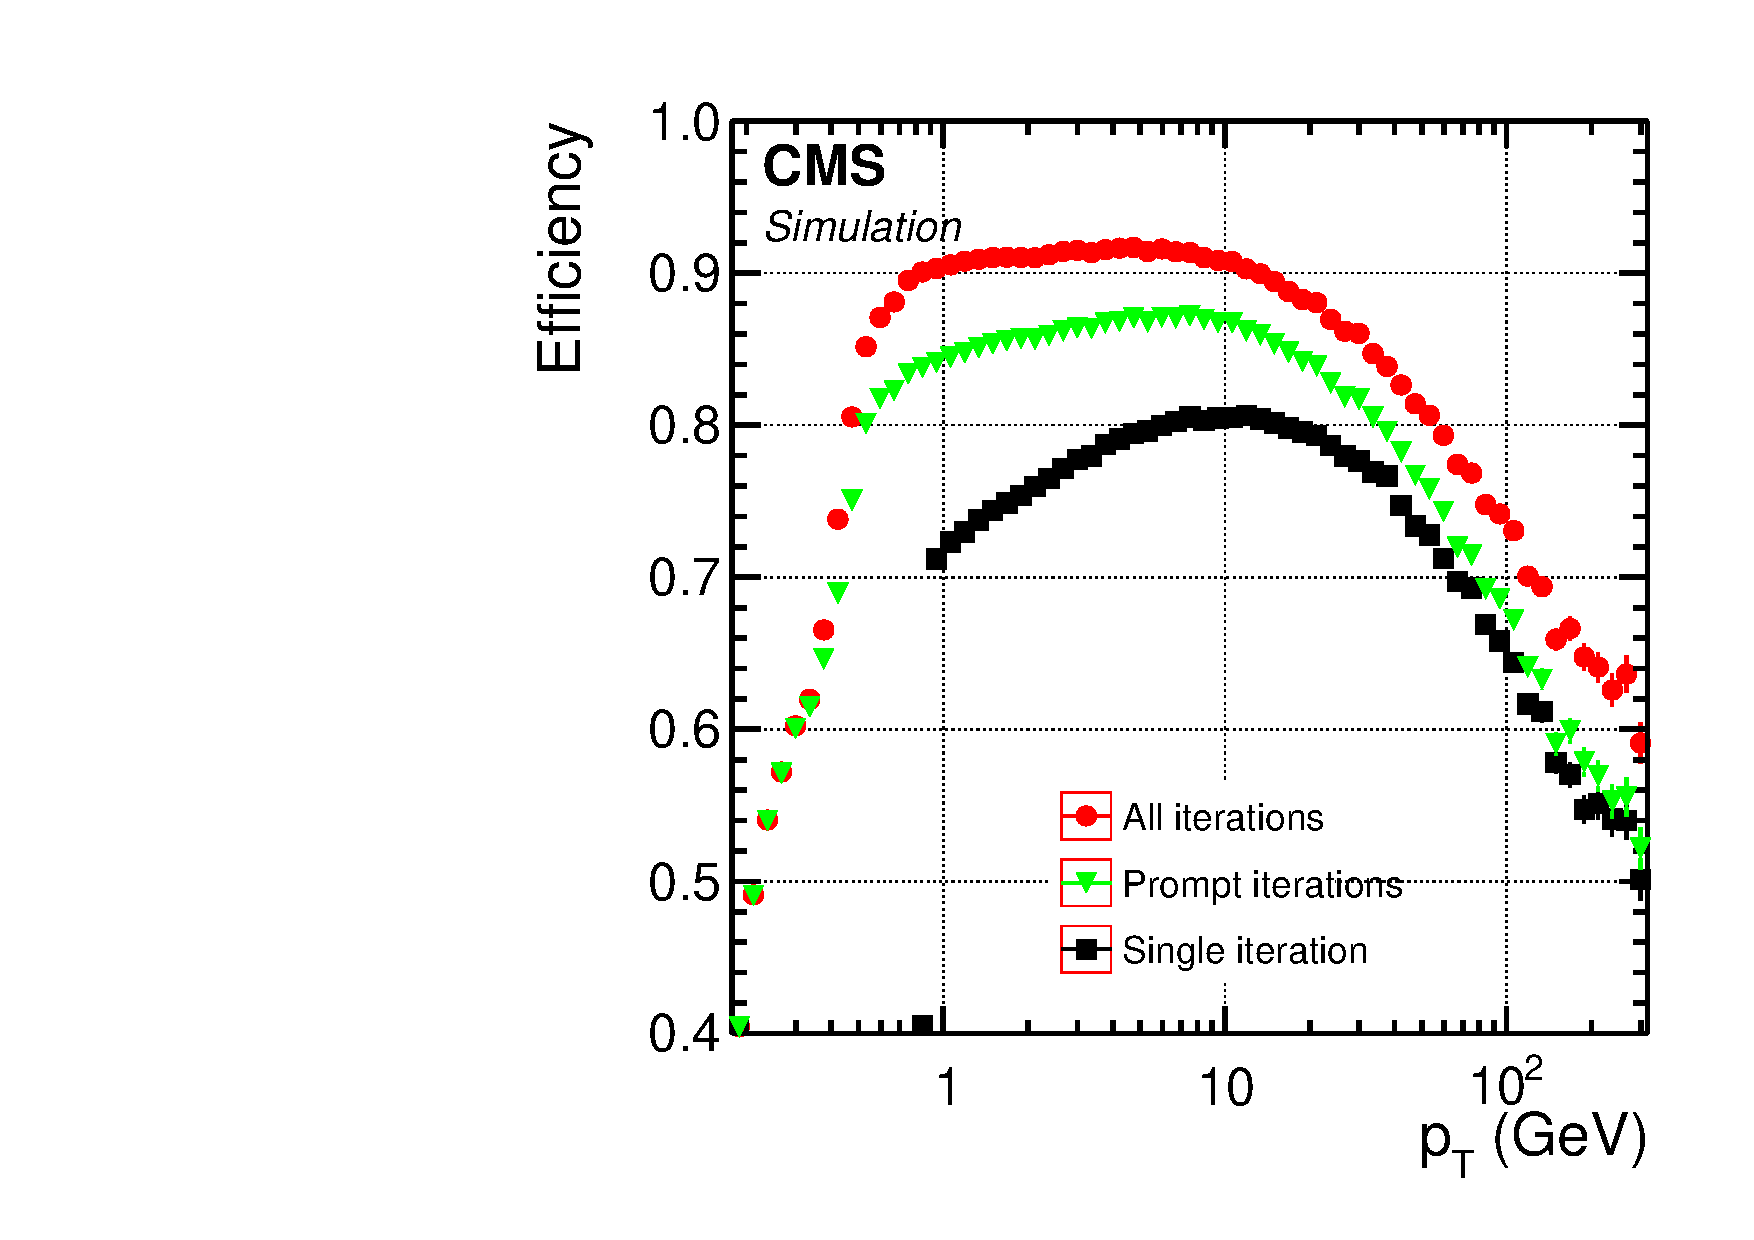
\includegraphics[width=0.45\textwidth]{object_reconstruction_and_selection/plots/pf_track_eff.pdf}
     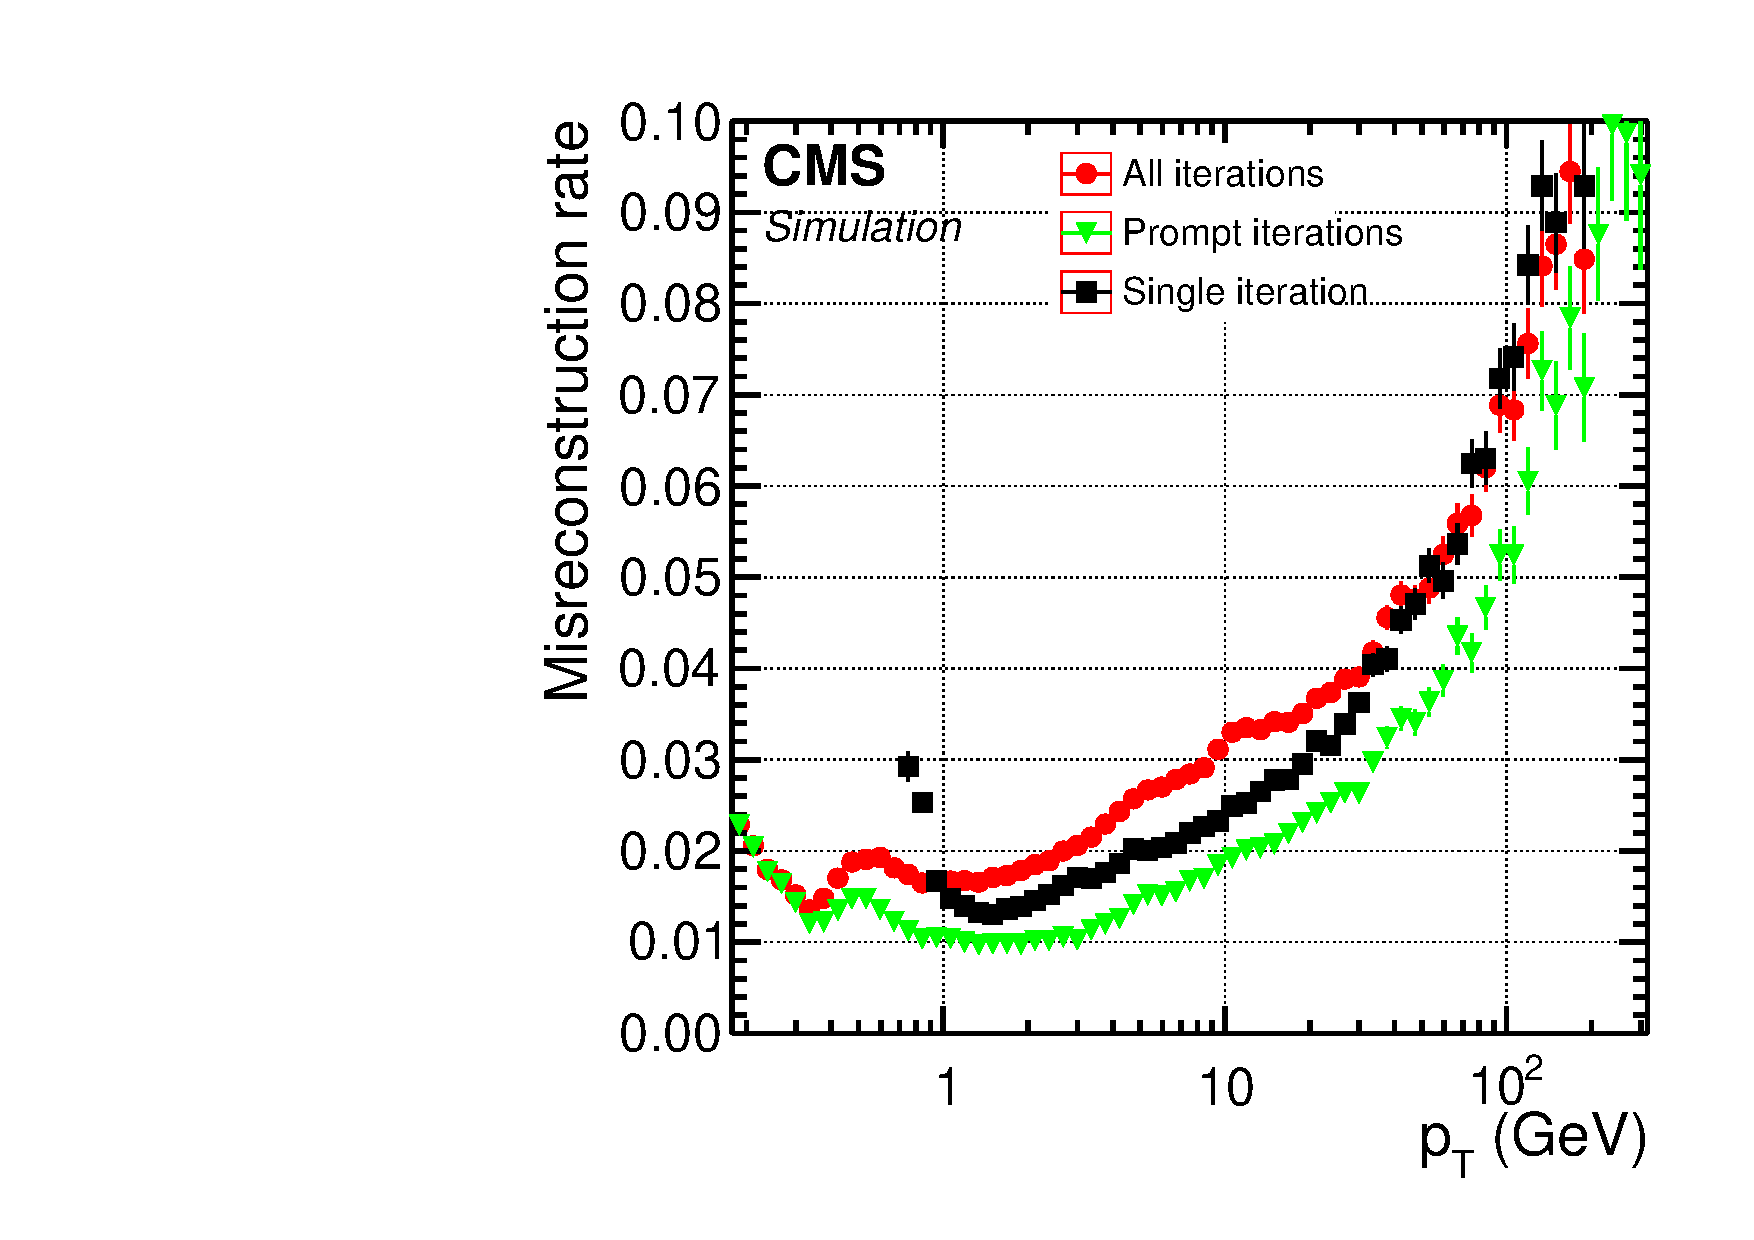
\includegraphics[width=0.45\textwidth]{object_reconstruction_and_selection/plots/pf_track_misId.pdf}
     \caption{
Efficiency (left) and misreconstruction rate (right) of the global combinatorial track finder (black squares) 
which is the first pass through the tracking algorithm. The prompt iterations of the tracking method (green 
triangles) show the results after all iterations based on seeds with at least one 
hit in the pixel detector are completed. The final results after all iterations (red circles) includes
iterations with displaced seeds. Efficiency and misreconstruction are plotted as a function 
of the track $\pt$, for charged hadrons in multijet events without pileup interactions. Only tracks with 
$\abs\eta < 2.5$ are considered. The efficiency 
is displayed for tracks originating from within 3.5 cm of the beam axis and $\pm$30 cm of the nominal 
centre of CMS along the beam axis.
     }
     \label{fig:kf_tracking}
\end{figure*}

Tracks which are likely associated with electrons receive special treatment in PF. Electrons
will often emit bremsstrahlung radiation while propagating through the tracker making their
tracks difficult to reconstruct because of the sudden kinks. 
When energetic photons are radiated from an electron, the pattern recognition in the KF algorithm
may have difficulty accommodating the sudden change in electron momentum. This can cause the track to 
be reconstructed with a small number of hits than would be associated with the true electron
path. A new collection of tracks is created based on a preselection on the number of hits and 
the fit $\chi^2$ for the reconstructed KF-based tracks. The new collection which is a subset of the
KF-based tracks are fit again with a Gaussian-sum filter (GSF)~\cite{gsf_electrons}. Instead of
modeling the energy loss of particles as a single gaussian probability density function (PDF) like the KF
algorithm does, the GSF models the energy loss as a mixture of multiple gaussiand PDFs. 
The GSF fitting algorithm is more adapted to electrons than the KF used in the iterative tracking.
It allows for sudden and substantial energy losses along the trajectory. The
additional freedom here allows much better fits for the electron-based tracks and provides
better estimates for the track origin, trajector towards the calorimeters, and $\pt$.

Muon tracks are built from a combination of the pixel and strip tracker information and the
muon spectrometer information. High purity muon hits in the muon spectrometer is granted by the 
calorimeters and the solenoid which absorb the vast majority of non-muon particles, except neutrinos, 
before reaching the muon spectrometer. There are three difference categories of muon tracks
reconstructed:
\begin{itemize}
\item Standalone muons are based on hits within each DT or CSC detector. Hits are clustered to form 
track segments that are used as seeds for the pattern recognition in the muon spectrometer to gather
other hits in the muon systems along the muon trajectory.
\item Global muons are reconstructed from a standalone-muon track which is matched to a track 
in the inner tracker. If the trajectory parameters of the two tracks propagated onto a common surface 
they are considered compatible and the hits from the inner track and from the standalone-muon track are combined and fit to form a global-muon track.
\item Tracker muons are built from an extrapolation of a track from the inner track system to a
single compatibe muon segment within the muon spectrometer system. The inner tracker-based track must have 
a $\pt > 0.5\GeV$ and a total momentum p in excess of 2.5 GeV.
\end{itemize}

About 99\% of the muons produced within the geometrical acceptance of the muon system are 
reconstructed either as a global muon or a tracker muon and very often as both.
For muons with $\pt > 200\GeV$ the momentum resolution, based on the inner track, is 
improved by the inclusion of the track extension to the muon system.
For muons with $\pt < 200\GeV$ the inner tracker already provides a precise measurement of 
their momentum.



\subsection{Particle Flow Energy Clusters}
Energy clusters make up the second basic building block to construct PF physics-objects. The PF energy
clustering algorithm which constructs the energy clusters serves multiple purposes. The energy clustering
is designed to:
\begin{itemize}
\item Detect and measure the energy and direction of stable neutral particles (photons and neutral hadrons)
\item Separate neutral particles from charged hadron energy deposits
\item Reconstruct and identify electrons and all accompanying bremsstrahlung photons
\item Assist the energy measurement of charged hadrons for which the track parameters were not 
determined accurately; this is primairly the case for low-quality and high-$\pt$ tracks
\end{itemize}
The clustering is performem separately in each subdetector, the ECAL barrel and end caps and HCAL barrel
and end caps with an aim of a high detection efficiency even for low-energy particles and the ability to 
separat close energy deposits. Clustering begins with seed hits which have an energy above the seed hit
threshold and an energy larger than the energy of the adjacent hits. In the ECAL barrel, the fine 
granularity of the ECAL allows
for the clustering to consider all eight adjacent hits, four on the sides and four on the corners.
The HCAL barrel has a more coarse granularity, so only the four adjacent sides are considered when
selecting a seed candidate. From the starting seed, topological clusters are grown outward by aggregating
hits with at least a corner in common with a cell already included in the cluster. Hits must have an energy
in excess of two times the subdetector noise level to be considered for clustering. The energy thresholds
for seeding a cluster and cluster inclusion threshold are in table~\ref{tab:pf_cluster_thresholds}.


\begin{table*}[htbp]
\centering
\begin{footnotesize}
%\begin{scriptsize}
\begin{tabular}{|l|cc|cc|}
\hline
        &       \multicolumn{2}{|c|}{ECAL}        &       \multicolumn{2}{|c|}{HCAL}        \\  %&   Preshower \\
        &   barrel  &   endcaps        &       barrel   &   endcaps        \\  %&    \\
\hline
Cell $E$ threshold (\MeV) & 80 & 300    &   800 &   800 \\   %& 0.06 \\
\hline
Seed Number closest cells   &   8 & 8   &   4 & 4 \\    %& 8 \\
Seed $E$ threshold (\MeV)   &  230  &  600  &  800  & 1100 \\    %& 0.12  \\
Seed $E_{\text{T}}$ threshold (\MeV)   &  0  &  150  & 0   & 0 \\    %& 0 \\
%\hline
%Gaussian width (cm)   &  1.5  &  1.5  &  10.0  & 10.0  \\    %& 0.2 \\
\hline
\end{tabular}
\end{footnotesize}
%\end{scriptsize}
\label{tab:pf_cluster_thresholds}
\caption{
The clustering parameters used for ECAL and HCAL energy deposit clustering. The ECAL endcap
requires an additional seed $E_{\text{T}}$ threshold because the detector noise
increases as a function of $\abs\eta$.
}
\end{table*}

Residual energy calibrations are applied to the ECAL and HCAL energy clusters. The calibrations are
designed to account for the effects of the hit energy thresholds which will always result in a 
smaller amount of energy being incorporated into a cluster than was measured by the detector
for a given single object.
In the ECAL, the residual energy calibration is determined from simulated single photon events.
This generic calibration is applied to all ECAL clusters prior to the hadron cluster calibration 
mentioned next. 

ECAL and HCAL energy clusters are linked together as a potential hadronicy decay energy deposit
if their positions in \etaphi overlap. For a hadronic decay, the total calorimeter response (ECAL + HCAL) depends on 
the fraction of the shower energy deposited in the ECAL, and is not linear with energy. The 
ECAL and HCAL cluster energies therefore need to be substantially recalibrated to get an 
estimate of the true hadron energy. Simulated single neutral hadrons, specifically single 
$\text{K}^{0}_{\text{L}}$s, are used for the hadronic decay response calibration seen for the
barrel in figure~\ref{fig:pf_calo_calib}. The applied calibrations in the left plot lead
to excellent agreement in the calorimeter response in the right plot. It is much harder to
make larger improvements in the energy resolution without actually changing the available
input calorimeter hit information granularity.


\begin{figure*}[htbp]
\centering
     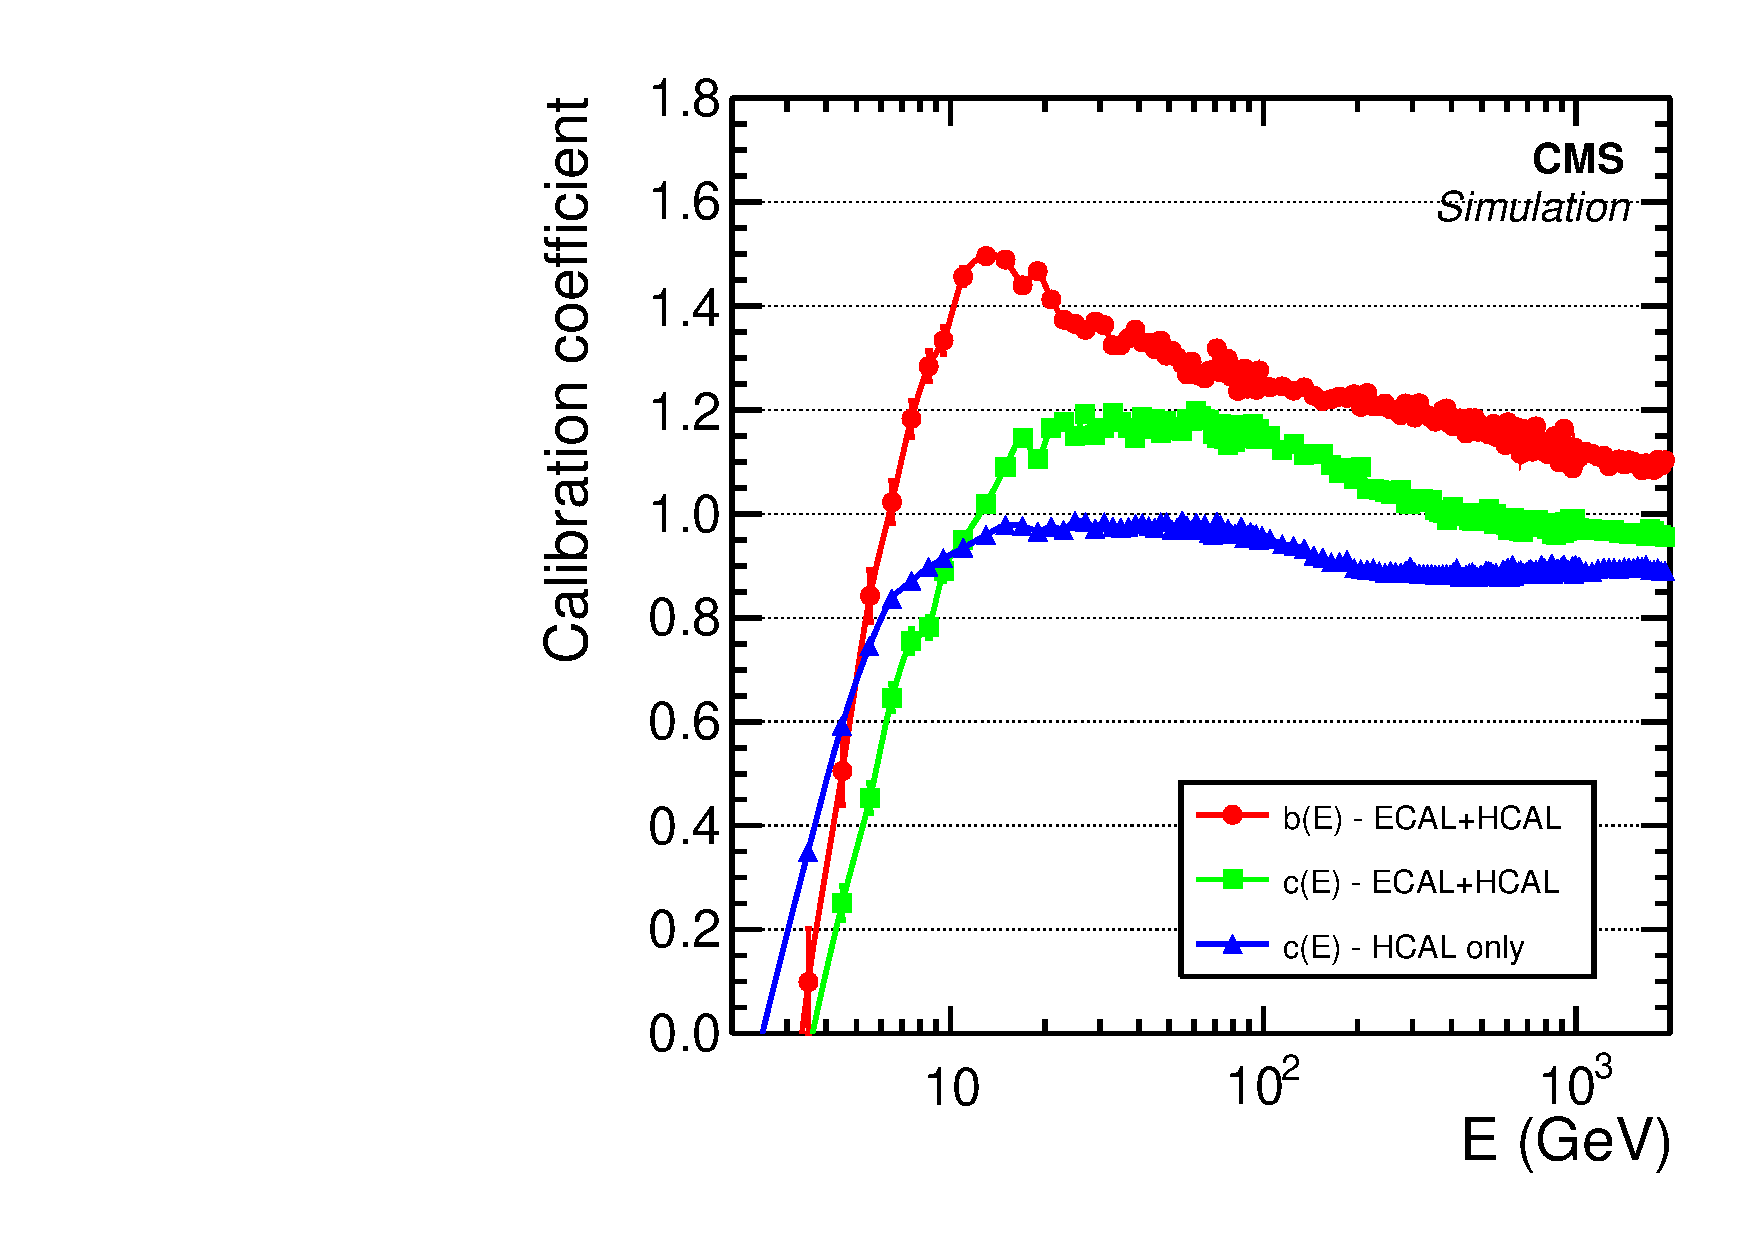
\includegraphics[width=0.45\textwidth]{object_reconstruction_and_selection/plots/calo_calibrations.pdf}
     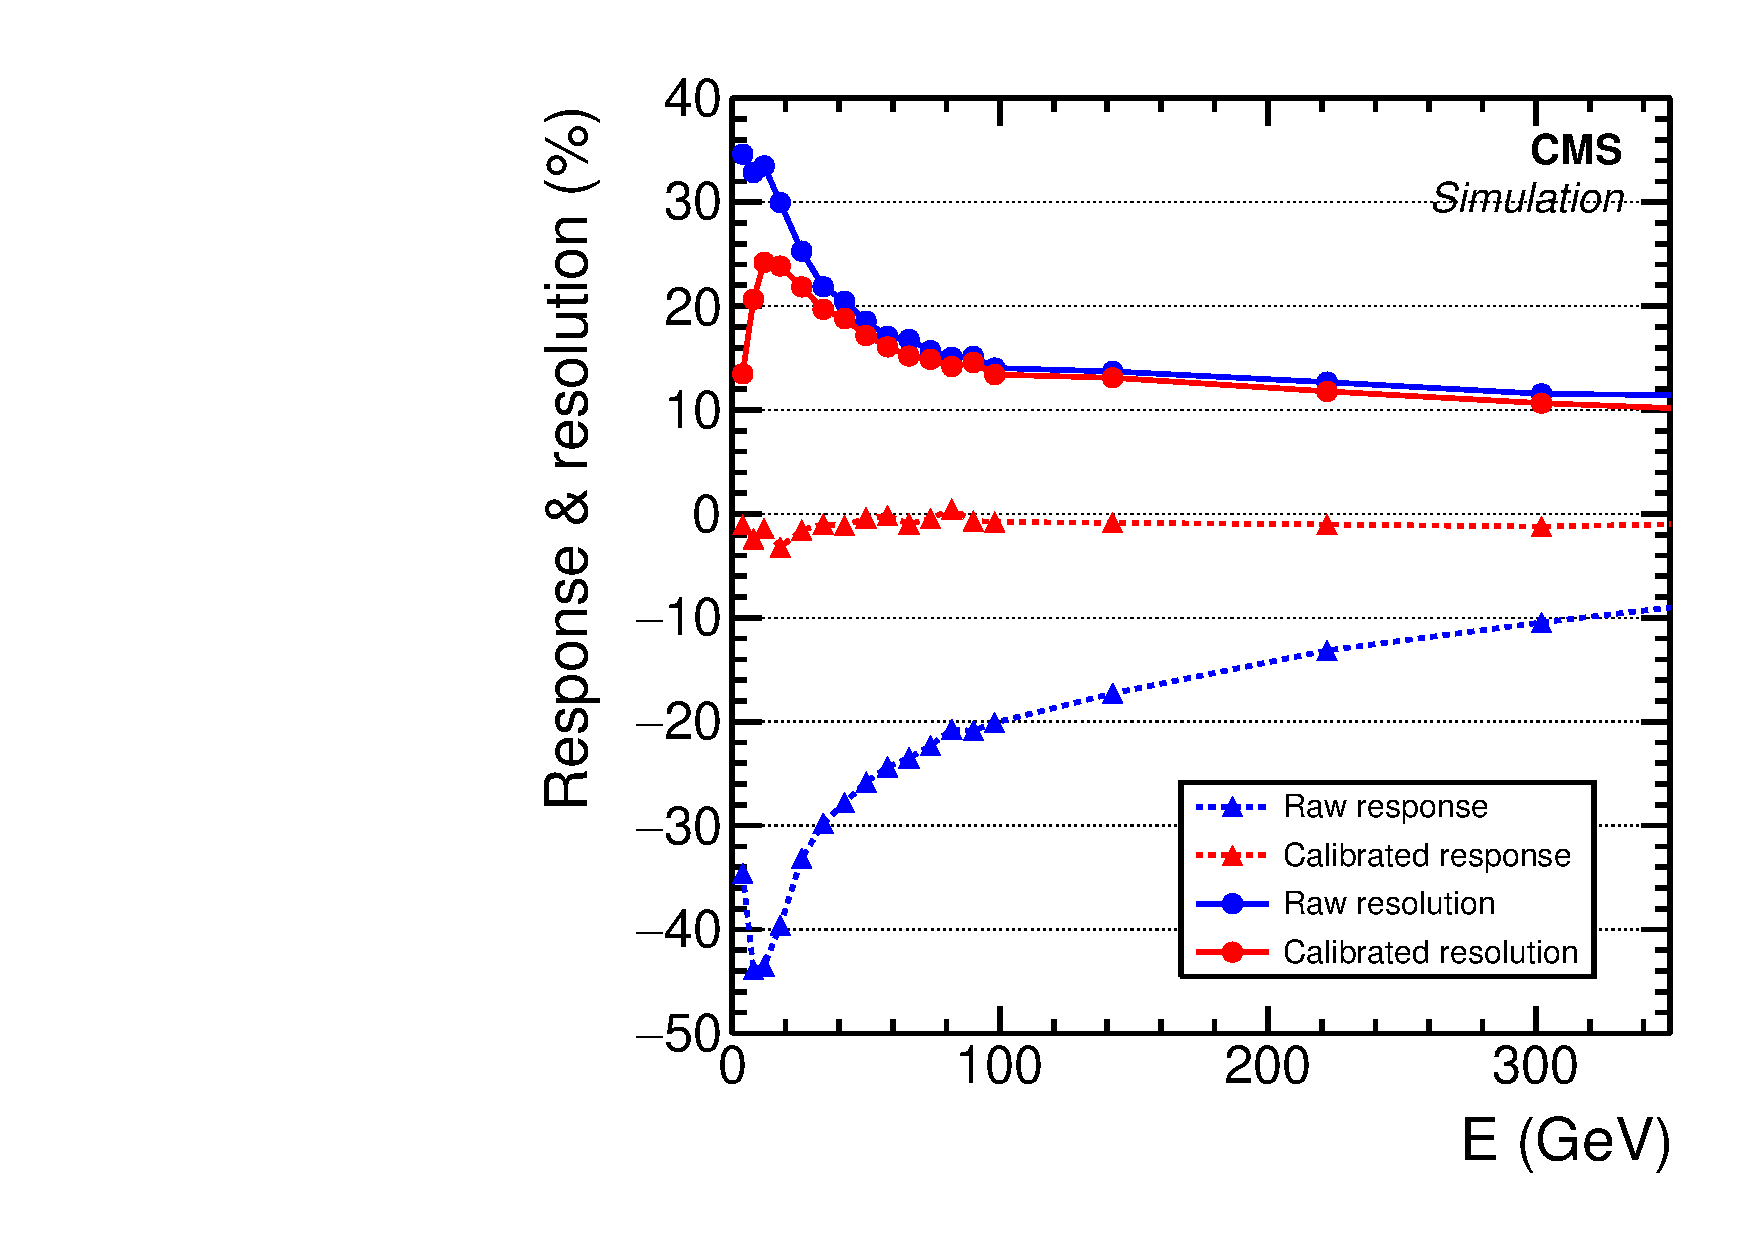
\includegraphics[width=0.45\textwidth]{object_reconstruction_and_selection/plots/calo_response_and_res.pdf}
     \caption{
(left) Calibration coefficients obtained from single $\text{K}^{0}_{\text{L}}$s in the barrel as a 
function of their true energy $E$. The blue triangles show the calibrations for hadrons depositing 
energy only in the HCAL. The red circles (green squares) show the ECAL (HCAL) calibration for hadrons
depositing energy in both the ECAL and HCAL.
(right) Relative raw (blue) and calibrated (red) energy response (dashed curves and triangles) and 
resolution (full curves and circles) for single $\text{K}^{0}_{\text{L}}$s in the barrel, as a 
function of their true energy $E$.
%Here the raw (calibrated) response and resolution are obtained by a Gaussian fit to the distribution of 
%the relative difference between the raw (calibrated) calorimetric energy and the true hadron energy.
     }
     \label{fig:pf_calo_calib}
\end{figure*}


In general, a given particle is expected to result in multiple PF elements (tracks and energy
clusters) in the various CMS subdetectors. The reconstruction of a particle first proceeds 
with a link algorithm that connects the PF elements from different subdetectors. For example,
tracks are linked to energy clusters if the extrapolated position of the track aligns within the
angular acceptance of an energy cluster in \etaphi. Energy clusters can be linked between subdetectors as mentioned
in the case of hadronic energy deposits above which span the ECAL and HCAL. A link is established
when the cluster position in the more granular calorimter, ECAL, is within the cluster envelope
in the less granular calorimeter, HCAL. Once PF elements are linked together they are referred to as a PF block which can contain 
elements associated either by a direct link or by an indirect link through common elements.
The link distance is defined as the distance between the extrapolated track position and the 
cluster position in the \etaphi plane.


\subsection{Particle Flow Candidates}
Particle Flow candidates are selected from the PF blocks based on designated quality cuts.


\subsubsection{Muons}
Isolated global muons are selected from the global muon track colletion by looking at the inner
tracker tracks and calorimeter 
energy deposits within a distance $\Delta \text{R} < 0.3$ to the muon trajectory. 
The sum of the $\pt$ of the tracks and of the ET of the energy deposits is required not to 
exceed 10\% of the muon $\pt$. This isolation criterion alone successfully reject hadrons that would
otherwise be misidentified as muons. No further selection is applied to these muon candidates.
If the muon track $\pt < 200\GeV$, then the momentum assigned to the muon PF candidate is that of 
the inner track. For muon tracks with $\pt > 200\GeV$, the momentum assigned is the momentum associated
with the smallest $\chi^2$ probability from these different track fits: tracker only, tracker and 
first muon detector plane, global, and global without the muon detector planes featuring a high occupancy.
The PF elements and blocks that make up a identified PF muon candidate masked against further processing
to prevent their inclusion in other PF candidates.

In these analyses, there are several additional criteria applied beyond that which is required to
be a PF candidate. These analyses use muons which pass two different PF muon identification working
points: \texttt{PF ID Loose} and \texttt{PF ID Medium}~\cite{sm-htt-2017}. The \texttt{PF ID Loose}
working point is only slightly tighter than the baseline criteria for a PF muon candidate; 
\texttt{PF ID Loose} must be either a global or a tracker PF muon. This selection is highly efficient
for prompt muons.

The \texttt{PF ID Medium} muon working point requires first that muons pass \texttt{PF ID Loose} then
applies additional track-quality and muon-quality requirements on the different muon tracks which are
linked to the PF muon candidate. The number of valide inner tracker
hits must be greater than 80\%. Additionally either one or the other of the following criteria must be met:
\begin{outline}
\1 Option 1 - ``Tight Segment Compatility''
    \2 Candidate has a segment compatility score of at least 0.451 which ensures that the 
track is reasonablly compatible with inner tracker-based track
\1 Option 2 - ``Good Global Muon'':
    \2 PF muon candidate is a global muon
    \2 The normalized track $\chi^2 < 3$
    \2 The compatibility $\chi^2$ between the standalone muon track and the inner tracker muon is
less than 12
    \2 The muon track kink-finder, which is desiged to remove muons produced from in-flight decays, 
must have a value less than 20
    \2 Candidate has a segment compatility score of at least 0.303 which is looser than the value
required in Option 1
\end{outline}
The \texttt{PF ID Medium} muon working is still very efficienct for prompt muon selection but
does bring some additional reduction in fake object selection which is helpful in the high
statistics $htt$ analysis. 


\subsubsection{Electrons and Prompt Photons}
Electron identification considers the PF blocks with linked inner tracker tracks and calorimeter
energy clusters. Because of bremsstrahlung radiation, it is common for electrons to 

Electron reconstruction is based on combined information from the inner tracker and the calori- meters. Due to the large amount of material in the tracker, electrons often emit bremsstrahlung photons and photons often convert to e+e− pairs

Isolated photon reconstruction is therefore conducted together with electron reconstruction. In a given PF block, an electron candidate is seeded from a GSF track, as described in section 3.2, provided that the corresponding ECAL cluster is not linked to three or more additional tracks. A photon candidate is seeded from an ECAL supercluster with ET larger than 10 GeV, with no link to a GSF track.

sum of the energies measured in the HCAL cells with a distance to the supercluster position smaller than 0.15 in the \etaphi plane must not exceed 10\% of the supercluster energy.

The final energy assignment for electrons is obtained from a combination of the corrected ECAL energy with the momentum of the GSF track and the electron direction is chosen to be that of the GSF track

Electron candidates must satisfy additional identification criteria. Specifically, up to fourteen variables — including the amount of energy radiated off the GSF track, the distance between the GSF track extrapolation to the ECAL entrance and the position of the ECAL seeding cluster, the ratio between the energies gathered in HCAL and ECAL by the track-cluster association process, and the KF and GSF track $\chi^2$ and numbers of hits — are combined in BDTs trained separately in the ECAL barrel and endcaps acceptance, and for isolated and nonisolated electrons.

Photon candidates are retained if they are isolated from other tracks and calorimeter clusters in the event, and if the ECAL cell energy distribution and the ratio between the HCAL and ECAL energies are compatible with those expected from a photon shower.



\subsubsection{Charged and Neutral Hadrons}

Once muons, electrons, and isolated photons are identified and removed from the PF blocks, the remaining particles to be identified are hadrons from jet fragmentation and hadronization. These particles may be detected as charged hadrons (π±, K±, or protons), neutral hadrons (e.g. KL0 or neutrons), nonisolated photons (e.g. from π0 decays), and more rarely additional muons (e.g. from early decays of charged hadrons).

The ECAL and HCAL clusters not linked to any track give rise to photons and neutral hadrons. Within the tracker acceptance (|η| < 2.5), all these ECAL clusters are turned into photons and all these HCAL clusters are turned into neutral hadrons. The precedence given in the ECAL to photons over neutral hadrons is justified by the observation that, in hadronic jets, 25\% of the jet energy is carried by photons, while neutral hadrons leave only 3% of the jet energy in the ECAL.

\subsection{Jets}

If the calibrated calorimetric energy is compatible with the sum of the track momenta, no neutral particle is identified.



\subsection{Taus}
\subsection{Missing Transverse Energy}

raw missing transverse momentum vector is defined in such a way as to balance the vectorial sum of the transverse momenta of all particles

\begin{equation}
\vec{p}^{\text{miss}}_{\text{T,PF}}(\text{raw}) = - \sum^{N_{\text{particles}}}_{i=1} \vec{p}_{\text{T},i}
\end{equation}

\pagebreak
\section{Object Identification and Selection}
\subsection{Muons}
\subsection{Electrons}
\subsection{Taus}
\subsection{b-jet ID and Secondary Vertex}

\section{Primary Vertex Reconstruction}




The reconstruction of observed and simulated events relies on the particle-flow (PF) algorithm~\cite{Sirunyan:2017ulk},
which combines the information from the CMS subdetectors to identify
and reconstruct the particles emerging from $\Pp\Pp$ collisions:
charged hadrons, neutral hadrons, photons, muons, and electrons.
Combinations of these PF objects are used to reconstruct
higher-level objects such as jets, $\tauh$ candidates, or
missing transverse energy.
The reconstructed vertex with the largest value of summed physics-object $\pt^2$ is taken to be the primary $\Pp\Pp$ interaction vertex. The physics objects are the objects constructed by a jet finding algorithm~\cite{Cacciari:2008gp,Cacciari:2011ma} applied to all charged tracks associated with the vertex, including tracks from lepton candidates, and the corresponding associated missing transverse energy.

Muons are identified with requirements on the quality of
the track reconstruction and on the number of measurements in the
tracker and the muon systems~\cite{Chatrchyan:2012xi}.
Electrons are identified with a multivariate discriminant
combining several quantities describing the track quality,
the shape of the energy deposits in the ECAL,
and the compatibility of the measurements from the tracker and the
ECAL~\cite{Khachatryan:2015hwa}.
To reject non-prompt or misidentified leptons, a relative lepton isolation is defined as:
\begin{equation}
I^{\ell} \equiv \frac{\sum_{charged}  \PT + \max\left( 0, \sum_{neutral}  \PT
                                         - \frac{1}{2} \sum_{charged, PU} \PT  \right )}{\PT^{\ell}}.
\label{eq:reconstruction_isolation}
\end{equation}
In this expression, $\sum_charged  \PT$ is the scalar sum of the
transverse energy of the charged particles originating from
the primary vertex and located in a cone of size
$\Delta R = \sqrt{\smash[b]{(\Delta \eta)^2 + (\Delta \phi)^2}} = 0.4$\,(0.3)
centered on the muon (electron) direction. The sum
$\sum_{neutral}  \PT$  represents
a similar quantity for neutral particles.
The contribution of photons and neutral hadrons originating from pileup vertices is estimated from the scalar sum of the transverse
energy of charged hadrons in the cone originating from pileup vertices,
$\sum_{charged, PU} \PT$. This sum is multiplied by a factor of
$1/2$, which corresponds approximately to the ratio of neutral to charged
hadron production in the hadronization process
of inelastic $\Pp\Pp$ collisions, as estimated from simulation.
The expression $\PT^{\ell}$ stands for the $\pt$ of the lepton. Isolation requirements used in this analysis, based on $I^{\ell}$, are listed in Table~\ref{tab:inclusive_selection}.

Jets are reconstructed with an anti-\kt clustering algorithm implemented
in the \FASTJET library~\cite{Cacciari:2011ma, Cacciari:fastjet2}.
It is based on the clustering of neutral and charged PF candidates within a distance parameter of 0.4. Charged PF candidates
not associated with the primary vertex of the interaction
are not considered when building jets. An offset correction is applied to jet energies to take into account the contribution from additional $\Pp\Pp$ interactions within the same or nearby bunch crossings. The energy of a jet is calibrated based on simulation and
data through correction factors~\cite{CMS-JME-10-011}.
In this analysis, jets are required to
have $\pt$ greater than 30\GeV and $\abs{\eta}$ less than 4.7, and
are separated from the selected leptons by a $\Delta R$ of at least 0.5.
The combined secondary vertex (CSV) algorithm is used to identify jets that are likely to originate from a b quark (``b jets"). The algorithm exploits the track-based lifetime information together with the secondary vertices associated with the jet to provide a likelihood ratio discriminator for the b jet identification. A set of $\pt$-dependent correction
factors are applied to simulated events to account for differences in the b tagging efficiency
between data and simulation. The working point chosen in this analysis gives an efficiency for real b jets of about 70\%, and for about 1\% of light flavor or quark jets being misidentified.

Hadronically decaying $\Pgt$ leptons
are reconstructed with the hadron-plus-strips (HPS)
algorithm~\cite{Khachatryan:2015dfa, CMS-PAS-TAU-16-002}, which is
seeded with anti-\kt jets.
The HPS algorithm reconstructs $\tauh$ candidates on the basis of the
number of tracks and of the number of ECAL strips in the $\eta$-$\phi$ plane with energy deposits, in the 1-prong,
1-prong + $\PGpz$(s), and 3-prong decay modes. A
multivariate (MVA) discriminator~\cite{Hocker:2007ht}, including isolation
and lifetime information, is used to reduce the rate for  quark- and gluon-initiated jets
to be identified as $\tauh$ candidates. The working point used in this analysis
has an efficiency of about 60\% for genuine $\tauh$,
with about 1\% misidentification rate for quark- and gluon-initiated jets, for a $\pt$ range typical of $\tauh$ originating from a $\PZ$ boson.
Electrons and muons misidentified as $\tauh$ candidates are suppressed using dedicated criteria
based on the consistency between the measurements in the tracker, the calorimeters, and the muon detectors~\cite{Khachatryan:2015dfa, CMS-PAS-TAU-16-002}.
The working points of these discriminators depend on the
decay channel studied.
The $\tauh$ energy scale in simulation is corrected per decay mode, on the basis of a measurement in $\PZ\to\Pgt\Pgt$ events. The rate and the
energy scale of electrons and muons misidentified as $\tauh$ candidates are also corrected in simulation, on the basis of a tag-and-probe measurement~\cite{CMS:2011aa} in $\PZ\to\ell\ell$ events.

All particles reconstructed in the event are used to determine the missing transverse energy,
\etvecmiss. The missing transverse momentum is defined as the negative vectorial sum of the transverse energy of
all PF candidates~\cite{Khachatryan:2014gga}. It is adjusted for the effect of jet energy corrections.
Corrections to the $\etvecmiss$ are applied to reduce the mismodeling of the simulated
$\PZ$+jets, $\PW$+jets and Higgs boson samples.
The corrections are applied to the simulated events on the basis of the vectorial difference
of the measured missing transverse energy and total transverse energy of neutrinos
originating from the decay of the $\PZ$, $\PW$, or Higgs boson. Their average effect is the reduction of the $\etvecmiss$ obtained from simulation by a few \GeV.

The visible mass of the $\Pgt\Pgt$ system, $\mvis$, can be used to separate
the $\PH\to \Pgt \Pgt$ signal events
from the large contribution of irreducible $\PZ \to \Pgt \Pgt$ events.
However, the neutrinos from the $\Pgt$ lepton decays carry a large fraction of
the $\Pgt$ lepton energy and reduce the discriminating power of this variable.
The \textsc{svfit} algorithm combines the \etvecmiss with the four-vectors of both $\Pgt$ candidates
to calculate a more accurate estimate of the mass of the parent boson, denoted as $\mtt$. The resolution of $\mtt$ is between 15 and 20\% depending on the $\Pgt\Pgt$ final state.
A detailed description of the algorithm can be found
in Ref.~\cite{Bianchini:2014vza}. Both variables are used in the analysis, as detailed in Section.~\ref{sec:categories}, and $\mvis$ is preferred over $\mtt$ when the background from $\PZ \to \ell\ell$ events is large.
